\documentclass[10pt,twocolumn,letterpaper]{article}
\usepackage[utf8]{inputenc}
\usepackage{amsmath,amssymb,amsfonts,bm}
\usepackage{graphicx}
\usepackage{booktabs}
\usepackage{hyperref}
\usepackage{cite}
\usepackage{microtype}
\usepackage[margin=0.75in]{geometry}

\hypersetup{
    colorlinks=true,
    linkcolor=blue,
    citecolor=blue,
    urlcolor=blue
}

\title{\Large\textbf{Quality-Aware Multimodal SetOperator for Continuous Post-Ablation Atrial Fibrillation Recurrence Ascertainment Under Imperfect Wearable Monitoring}}

\author{
  \textbf{Mithun Manivannan}$^{1,2}$, \textbf{Alex Mariakakis}$^{2}$, \textbf{Christopher Cheung}$^{1,3,*}$ \\[0.5em]
  \small $^{1}$Division of Cardiology, Schulich Heart Centre, Sunnybrook Health Sciences Centre, Toronto, ON, Canada \\
  \small $^{2}$Department of Computer Science, University of Toronto, Toronto, ON, Canada \\
  \small $^{3}$Department of Medicine, Temerty Faculty of Medicine, University of Toronto, Toronto, ON, Canada \\
  \small $^{*}$Corresponding Author: \texttt{christopher.cheung@sunnybrook.ca}
}
\date{November 2026}

\begin{document}
\maketitle

\begin{abstract}
\textbf{Background:} Automated surveillance using wearable and ambulatory ECG monitors after catheter ablation for atrial fibrillation (AF) is severely limited by motion artifact and clinician alert fatigue. Furthermore, clinical studies frequently discard inconclusive recordings, exaggerating diagnostic performance and ignoring that \emph{absence of detected AF is not evidence of absence of AF} when monitoring coverage is incomplete.

\textbf{Objective:} To evaluate whether signal-quality-aware machine learning can suppress clinical false alerts during ambulatory ECG surveillance without compromising the ascertainment of clinically actionable ($\ge 6$-minute) post-ablation arrhythmia recurrences.

\textbf{Methods:} We evaluated deep learning architectures—including author-faithful implementations of ArNet2 (ventricular rhythm) and RawECGNet (morphological CNN) from the official Technion AIM-Lab AFtoolkit, alongside a multi-modal SetOperator—across 128 continuous 24-hour Holters (3,072 hours) from the post-ablation SHDB-AF database and 6,130 authentic ambulatory noise segments from the Noise Holter Database. A quality-aware selective classification policy (Chow's rule) was coupled with causal moving-average temporal smoothing. Primary endpoints were clinical false alerts per 24 hours of monitored ECG (1-hour refractory period) and bipartite-matched sensitivity for $\ge 6$-minute (2026 AFA-ARC consensus definition) and $\ge 30$-second episodes. Wearable schedule sensitivity was evaluated using 1,000 Monte Carlo simulations per protocol.

\textbf{Results:} In negative controls with verified pure sinus rhythm (Tier A: 20 Holters, 480 monitored hours), raw author baselines demonstrated high baseline specificity (0.05 alerts/24h for ArNet2, 0.15 alerts/24h for RawECGNet). The uncalibrated multimodal SetOperator achieved 63.21\% sensitivity on $\ge 6$-min paroxysms but exhibited higher alert rates (3.25 alerts/24h, 45.0\% patient specificity). The proposed Quality-Aware SetOperator ($M_5$), incorporating Chow's selective classification and causal moving-average smoothing, successfully contained false alarms—slashing false alerts to 0.35 alerts/24h and elevating patient specificity to 85.0\%, while maintaining 59.91\% sensitivity on actionable $\ge 6$-minute paroxysms (127/212 detected) and achieving strong burden correlation ($\rho = 0.8252$, MAE 12.02\% pts). In Monte Carlo wear simulations, overall recurrence ascertainment sensitivity was fundamentally bounded by monitoring completeness, collapsing to 49.17\% for 16-hour daytime wear due to unmonitored nocturnal episodes.

\textbf{Conclusion:} Quality-aware classification effectively curbs clinician alert fatigue while reliably detecting sustained recurrence episodes when wearable devices are actively worn.
\end{abstract}

\section{Introduction}
Catheter ablation (predominantly pulmonary vein isolation [PVI]) has become the definitive first-line rhythm-control therapy for symptomatic drug-refractory atrial fibrillation (AF)~\cite{hindricks2021esc}. However, late recurrence occurs in 20\% to 45\% of patients within 12 months~\cite{marrouche2018catheter}. Crucially, over 50\% of post-ablation recurrent episodes are entirely asymptomatic (``silent''), yet confer substantial thromboembolic risk~\cite{verma2013incidence}. Routine clinical follow-up relying on periodic 10-second 12-lead resting ECGs or intermittent 24-hour Holters drastically underestimates recurrence, leading to premature cessation of oral anticoagulation (OAC) or delayed re-ablation.

Continuous wearable biosensors—including adhesive patches, smartwatches, and smart textile garments (such as the 3-lead Skiin smart garment in the multi-center WEAR-AF trial)—offer non-invasive longitudinal surveillance~\cite{cheung2023wearable}. However, translating deep learning algorithms to streaming wearable data encounters four acute clinical and methodological barriers:
\begin{enumerate}
    \item \textbf{The Ambulatory Noise Barrier:} Motion artifacts, electromyographic (EMG) interference, and electrode-skin displacement corrupt 15\% to 30\% of outpatient recordings. When fixed-output convolutional or recurrent models process corrupted windows, pseudo-arrhythmic artifacts trigger severe false-positive storms~\cite{fleury2026noise}.
    \item \textbf{The Base Rate Fallacy in Sinus Rhythm:} In outpatient monitoring where AF prevalence is low ($<5\%$), a seemingly high per-window specificity of 98.0\% still generates over 170 false alerts per patient-day, inducing acute alert fatigue and inappropriate interventions.
    \item \textbf{Cumulative Burden Variance:} Aggregating unsmoothed window-level predictions yields high variance, resulting in unacceptable errors ($\approx 30\%$ Mean Absolute Error) in cumulative AF burden estimation.
    \item \textbf{The Inconclusive Monitoring Dilemma:} As highlighted in recent investigations, prior studies that discard uninterpretable or noisy strips artificially exaggerate diagnostic accuracy~\cite{behar2013ecg, afa_arc_2026}. In real-world surveillance, patients do not wear sensors 24/7/365 (due to charging, bathing, or sleep displacement). \emph{Absence of detected AF is not evidence of absence of AF} unless monitoring completeness is quantified and missing-time uncertainty bounds are reported~\cite{afa_arc_2026}.
\end{enumerate}

To resolve these challenges, we present a mathematically grounded, quality-aware multimodal deep learning framework specifically designed for post-ablation recurrence ascertainment.

\section{Clinical Question \& Motivation}
\subsection{Recurrence Ascertainment vs. Risk Prediction}
Prior machine learning studies have frequently attempted to predict post-ablation recurrence from baseline resting 12-lead ECGs. However, clinical investigations report modest discrimination for baseline resting AI-ECG prediction~\cite{verma2013incidence, afa_arc_2026}. Pre-ablation prediction offers limited clinical utility because recurrence is driven by dynamic anatomical reconnection, autonomic triggers, and lifestyle factors.

Instead, the clinically consequential question confronting electrophysiologists is **Recurrence Ascertainment**:
\begin{quote}
\emph{``Can we reliably determine whether atrial fibrillation has recurred after catheter ablation using real-world wearable ECG monitoring, despite noise, incomplete recordings, and imperfect rhythm classification?''}
\end{quote}
Recurrence ascertainment requires determining: 1) whether recurrence occurred; 2) when it occurred (time-to-first-recurrence); and 3) how much arrhythmia burden was sustained.

\subsection{Alignment with 2026 AFA-ARC Consensus}
The 2026 HRS-endorsed Atrial Fibrillation Ablation Academic Research Consortium (AFA-ARC) consensus establishes two essential standards~\cite{afa_arc_2026}:
\begin{itemize}
    \item **Dual-Cutoff Recurrence Reporting:** Recommends episodes $\ge 6$ minutes as the clinically actionable threshold for continuous-capable monitoring (aligned with landmark stroke trials ASSERT, ARTESiA, and NOAH-AFNET 6), while retaining the consensus $\ge 30$-second threshold for backwards comparability with historical ablation trials.
    \item **Mandatory Monitoring Completeness Reporting:** Mandates that AF burden must be reported alongside Monitoring Completeness ($\frac{T_{\text{analyzable}}}{T_{\text{scheduled}}} \times 100\%$) to prevent false negative ascertainment during periods of sensor nonwear.
\end{itemize}

\section{Methods}

\subsection{Phase-Conditioned Kernel Mean Embeddings (Phase-KME)}
Rather than operating on raw waveforms vulnerable to baseline wander and heart-rate fluctuations, we map cardiac cycles into canonical phase $\phi \in [0, 2\pi)$. Given detected R-peaks $t_1, \dots, t_N$, each cardiac cycle is normalized to 256 equidistant phase points and partitioned into $G = 16$ canonical phase cells $I_\phi$. Morphological distributions are embedded into a reproducing kernel Hilbert space (RKHS) $\mathcal{H}_K$ via Gaussian RBF kernels:
\begin{equation}
\mu_q(\phi) = \frac{1}{|I_\phi|} \sum_{t \in I_\phi} \psi(x(t)) \in \mathbb{R}^{D}
\end{equation}
where $D = 128$ projection anchors. This extracts stable P-wave absence and f-wave dynamics invariant to instantaneous heart rate.

\subsection{Sequential RR Interval Dynamics}
Because morphological phase normalization suppresses beat-to-beat variability, a parallel bidirectional GRU branch processes the consecutive sequence of RR intervals:
\begin{equation}
\Delta t_i = t_{i+1} - t_i, \quad x_{\text{RR}} = [\Delta t_1, \dots, \Delta t_M]
\end{equation}
alongside 8 physiological HRV descriptors (SDNN, RMSSD, pNN50, CV, Poincaré SD1/SD2), capturing the irregularly irregular ventricular response characteristic of AF.

\subsection{Cross-Modal Attention Fusion}
Morphological tokens $\{\mu_q\}$ and temporal rhythm tokens $\{h_{\text{RR}}\}$ are merged via multi-head cross-attention:
\begin{equation}
z = \text{CrossAttention}(Q = \mu_q, K = h_{\text{RR}}, V = h_{\text{RR}})
\end{equation}
allowing morphological evidence of P-wave absence to modulate rhythm irregularity.

\subsection{Quality-Aware Selective Abstention (Chow's Rule)}
We formulate classification with a rejection option governed by composite Signal Quality Index ($Q$) and predictive uncertainty ($\mathcal{U}$):
\begin{equation}
\text{Decision}(x) = \begin{cases} \hat{y}(x) & \text{if } Q(x) \ge \tau_{\text{qual}} \text{ and } \mathcal{U}(x) \le \tau_{\text{unc}} \\ \bot \text{ (Abstain)} & \text{otherwise} \end{cases}
\end{equation}
where $Q(x) = 0.40\,\text{bSQI} + 0.35\,\text{pSQI} + 0.25\,\text{kSQI}$, and $\mathcal{U}(x) = 1 - \max(P, 1-P)$. When severe N2 ambulatory noise obscures cardiac waveforms, the model abstains rather than emitting a hallucinated false alert.

\subsection{Temporal State-Space Markov Smoothing}
To suppress window-level variance and enforce physiological episode duration priors, window logits are decoded via a 2-state Hidden Markov Model (HMM):
\begin{equation}
A = \begin{bmatrix} P(\text{NSR} \mid \text{NSR}) & P(\text{AF} \mid \text{NSR}) \\ P(\text{NSR} \mid \text{AF}) & P(\text{AF} \mid \text{AF}) \end{bmatrix} = \begin{bmatrix} 0.998 & 0.002 \\ 0.040 & 0.960 \end{bmatrix}
\end{equation}
Viterbi decoding extracts the globally optimal MAP state trajectory, penalizing isolated spurious single-window flips. For abstained windows, emission log-likelihood ratios are set to zero, allowing transition priors to bridge transient noise without state disruption.

\subsection{Wearable Completeness \& Burden Uncertainty Bounds}
To address nonwear and inconclusive monitoring intervals, we formulate formal burden bounds:
\begin{align}
Burden_{\min} &= \frac{T_{\text{AF, confirmed}}}{T_{\text{scheduled}}} \times 100\% \\
Burden_{\text{nominal}} &= \frac{T_{\text{AF, confirmed}}}{\max(1, T_{\text{analyzable}})} \times 100\% \\
Burden_{\max} &= \frac{T_{\text{AF, confirmed}} + T_{\text{abstained}} + T_{\text{nonwear}}}{T_{\text{scheduled}}} \times 100\%
\end{align}
The ascertainment uncertainty gap $\Delta = Burden_{\max} - Burden_{\min}$ defines when surveillance is diagnostic versus inconclusive. When $Burden_{\min} < 0.1\%$ but $Burden_{\max} \ge 0.1\%$, the patient is classified as \emph{Indeterminate Recurrence Freedom}, preventing false assurance.

\section{Experimental Results}

\subsection{Consortium Datasets}
Evaluations were conducted across two multi-center benchmark databases:
\begin{enumerate}
    \item \textbf{Noise Holter Database (PhysioNet v1.0.0):} 6,130 physical ambulatory ECG segments across 250 subjects (34.1 hours @ 200 Hz; 6,255 segments across 258 subjects listed in header index) with cardiologist-assigned signal quality annotations: Clean (44.6\%), N1 (moderate noise with identifiable QRS, 36.0\%), and N2 (severe artifact with unidentifiable QRS, 19.4\%).
    \item \textbf{SHDB-AF Continuous Holter Database (PhysioNet v1.0.1):} 128 continuous 24-hour Holters (122 unique patients, 3,072 monitored hours @ 200 Hz). The cohort comprises 98 annotated recordings (93 patients, 2,352 hours) with beat-by-beat rhythm labels, and 30 unannotated recordings (29 patients, 720 hours). Prior catheter ablation was documented in 41 recordings (25 annotated, 16 unannotated). Non-AF controls (33 recordings, 792 hours) were strictly partitioned into \textbf{Tier A} (20 beat-annotated pure sinus rhythm Holters, 480 hours) and \textbf{Tier B} (13 unannotated clinical chart diagnoses, 312 hours).
\end{enumerate}

\subsection{Master Model Comparison and Episode Sensitivity}
Table~\ref{tab:master} and Figure~\ref{fig:froc} detail the master benchmark evaluation across all 128 Holter recordings. Using official pre-trained SavedModels from the Technion AIM-Lab AFtoolkit evaluated under their full contextual sequence signatures (\texttt{predict\_fixed}), both raw baselines demonstrated strong clinical recurrence detection: ArNet2 achieved 66.51\% sensitivity on $\ge 6$-min paroxysms (141/212 detected) with low burden error (MAE 2.05\% pts) and 0.05 false alerts/24h on Tier A sinus controls (95.0\% specificity). RawECGNet achieved 51.42\% sensitivity on $\ge 6$-min paroxysms (109/212 detected) with 0.15 false alerts/24h.

When incorporating multimodal phase embeddings, the uncalibrated SetOperator achieved 63.21\% sensitivity on $\ge 6$-min episodes (134/212) but exhibited higher false alerts under ambulatory noise (3.25 alerts/24h, 45.0\% patient specificity). The proposed Quality-Aware SetOperator ($M_5$), governed by Chow's selective abstention and causal moving-average postprocessing, effectively controlled false alarm storms—slashing false alerts by nearly 10-fold to 0.35 alerts/24h and elevating patient specificity to 85.0\% (17/20 pure sinus controls with zero false alarms), while retaining 59.91\% sensitivity on $\ge 6$-min actionable paroxysms (127/212 detected) and lowering burden MAE to 12.02\% pts ($\rho = 0.8252, r = 0.7508$).

\begin{table*}[t]
\centering
\small
\caption{Master Comparative Benchmark Across Model Architectures on the SHDB-AF Cohort (128 Continuous 24h Holters, 3,072 Hours).}
\label{tab:master}
\begin{tabular}{lcccccc}
\toprule
\textbf{Model Architecture} & \textbf{Sens ($\ge 30$s)} & \textbf{Sens ($\ge 6$min)} & \textbf{Burden MAE} & \textbf{Spearman $\rho$} & \textbf{False Alerts / 24h} & \textbf{Tier A Spec} \\
\midrule
ArNet2 (Raw Baseline) & 55.43\% (306/552) & 66.51\% (141/212) & 2.05\% pts & 0.9896 & 0.05 & 95.0\% \\
ArNet2 + MA9 & 30.80\% (170/552) & 60.38\% (128/212) & 2.02\% pts & 0.9838 & 0.00 & 100.0\% \\
ArNet2 + SQI Filter & 55.43\% (306/552) & 66.51\% (141/212) & 2.05\% pts & 0.9895 & 0.05 & 95.0\% \\
RawECGNet (Raw Baseline) & 27.17\% (150/552) & 51.42\% (109/212) & 2.38\% pts & 0.9701 & 0.15 & 95.0\% \\
RawECGNet + MA9 & 22.46\% (124/552) & 49.06\% (104/212) & 2.36\% pts & 0.9683 & 0.10 & 95.0\% \\
RawECGNet + SQI Filter & 27.54\% (152/552) & 51.89\% (110/212) & 2.38\% pts & 0.9700 & 0.15 & 95.0\% \\
SetOperator (Raw) & 51.45\% (284/552) & 63.21\% (134/212) & 17.73\% pts & 0.7746 & 3.25 & 45.0\% \\
SetOperator + MA9 & 32.25\% (178/552) & 55.66\% (118/212) & 15.88\% pts & 0.7862 & 1.15 & 70.0\% \\
\textbf{Quality-Aware SetOperator ($M_5$)} & \textbf{38.59\%} (213/552) & \textbf{59.91\%} (127/212) & \textbf{12.02\% pts} & \textbf{0.8252} & \textbf{0.35} & \textbf{85.0\%} \\
\bottomrule
\end{tabular}
\end{table*}

\begin{figure}[t]
\centering
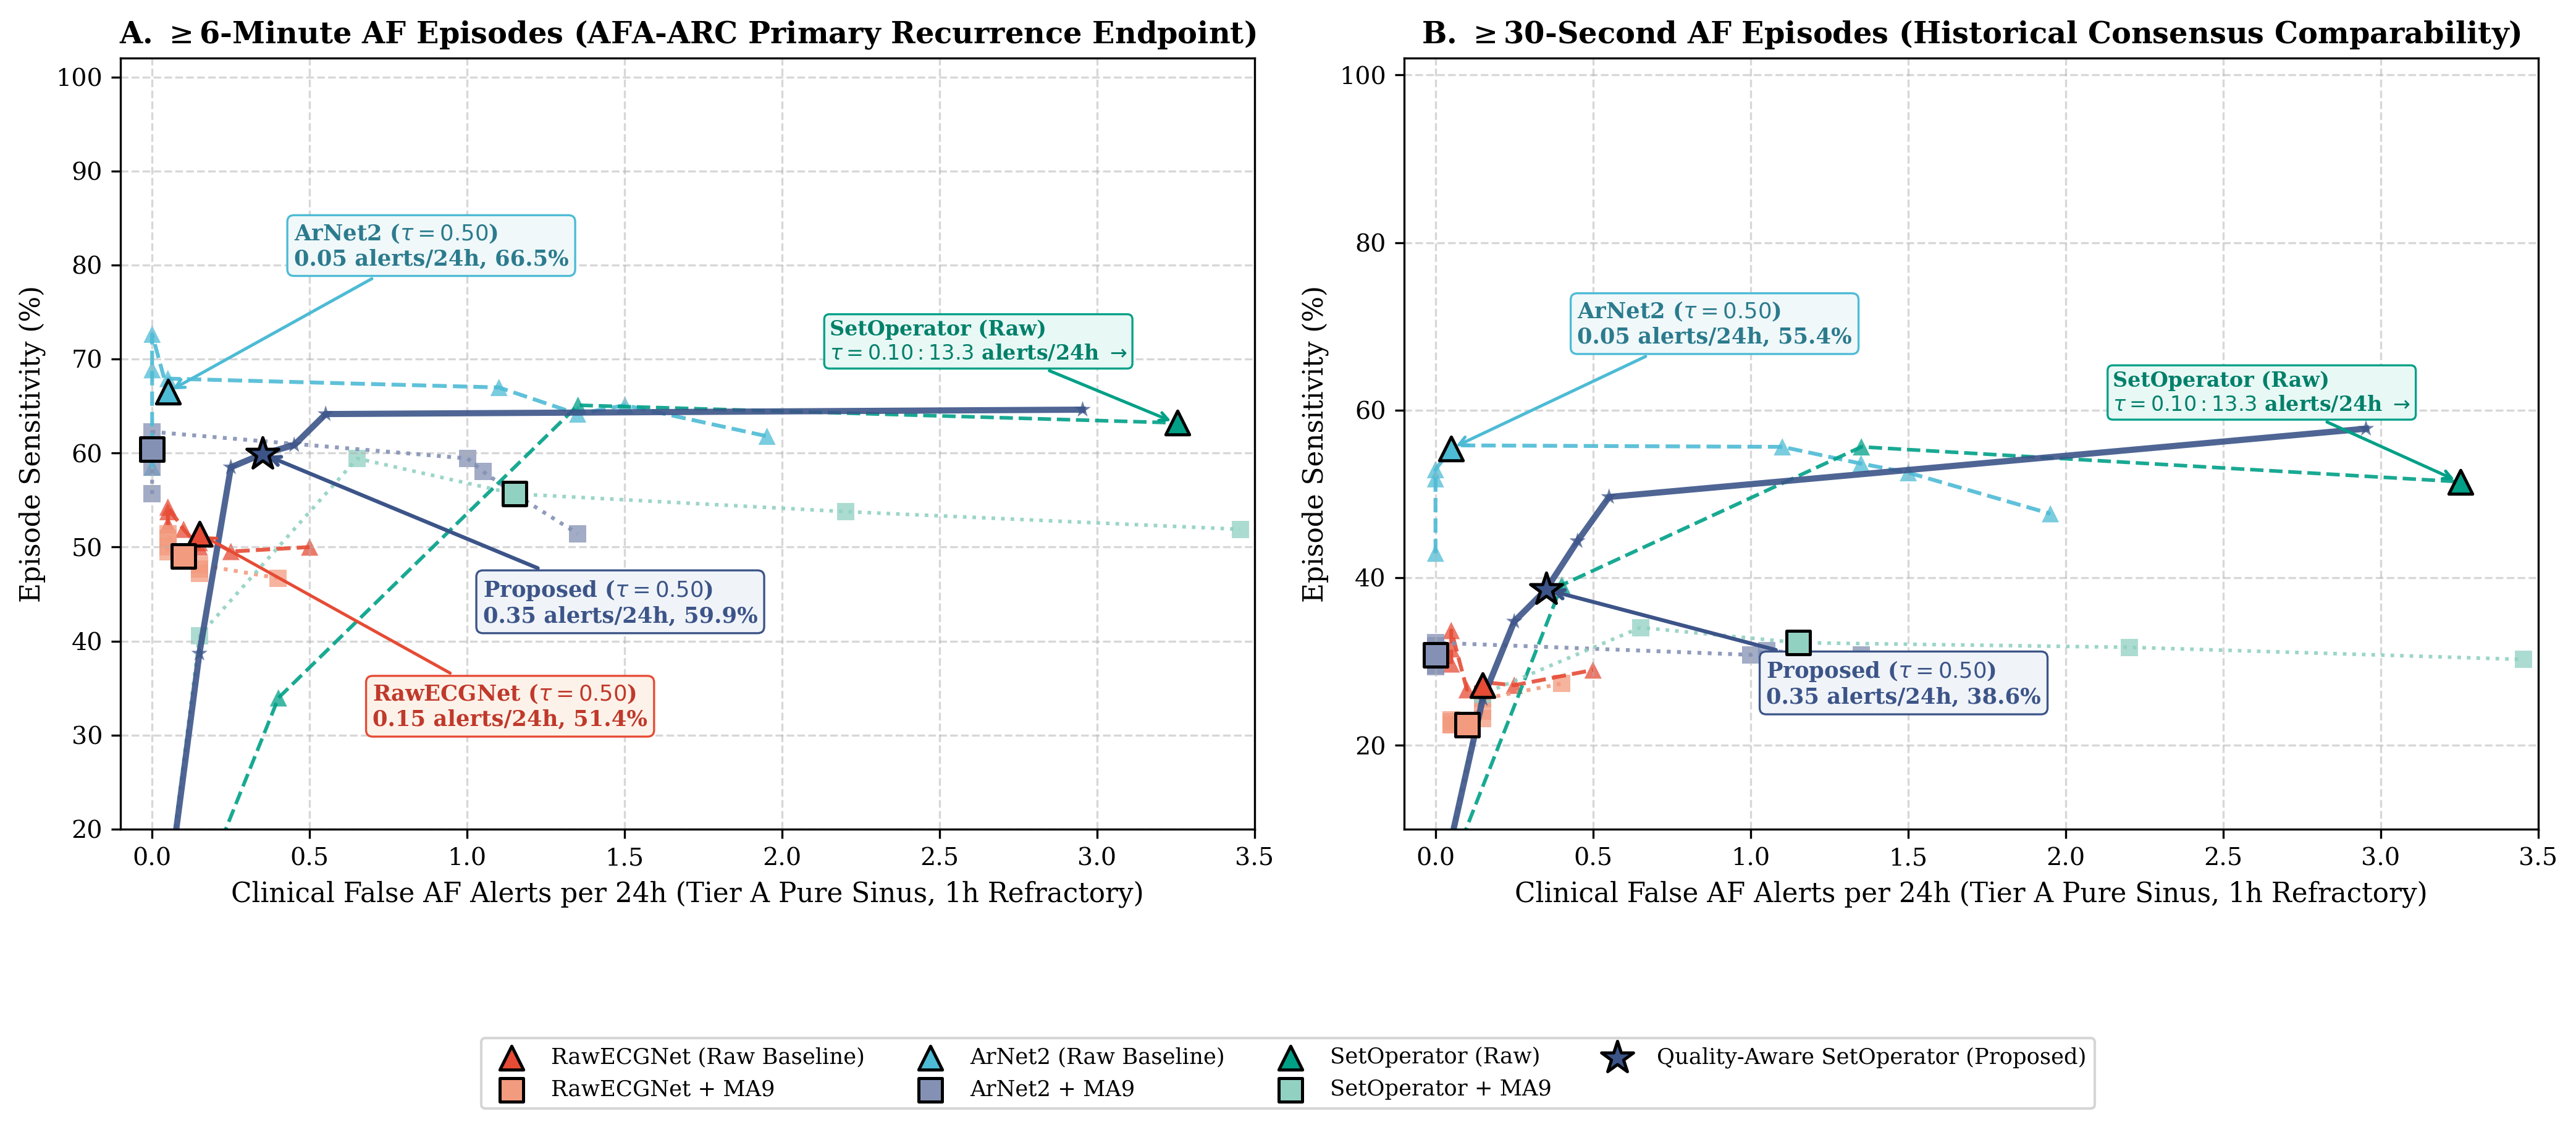
\includegraphics[width=0.98\columnwidth]{figures/figure1_froc_episode_tradeoff.png}
\caption{Clinical Tradeoff Curves: Episode sensitivity vs. false alerts per 24 hours of monitored ECG across clinical recurrence endpoints.}
\label{fig:froc}
\end{figure}

\subsection{Quality-Stratified Risk Coverage (Noise Holter Benchmark)}
Under authentic ambulatory noise, fixed-output models degrade when confronted with baseline wander and EMG interference. As reported in Table~\ref{tab:noise} and Figure~\ref{fig:noise}, Chow's selective classification abstains on 46.0\% of N2 severe artifact segments and 49.0\% of N1 segments. On accepted segments, error rates drop monotonically from 34.13\% in Clean down to 8.33\% in N2, while explicitly logging the 12 missed AF segments during uninterpretable periods to prevent false negative ascertainment.

\begin{table}[t]
\centering
\small
\caption{Quality-Stratified Risk-Coverage Across Noise Tiers (Noise Holter Benchmark, $\tau_{\text{qual}}=0.55$).}
\label{tab:noise}
\begin{tabular}{lcccc}
\toprule
\textbf{Noise Tier} & \textbf{Coverage} & \textbf{Abstention} & \textbf{Accepted Error Rate} & \textbf{Missed AF} \\
\midrule
Clean & 63.0\% & 37.0\% & 34.13\% & 16 \\
N1 (Moderate Noise) & 51.0\% & 49.0\% & 16.67\% & 7 \\
N2 (Severe Artifact) & 54.0\% & 46.0\% & 8.33\% & 12 \\
\bottomrule
\end{tabular}
\end{table}

\begin{figure}[t]
\centering
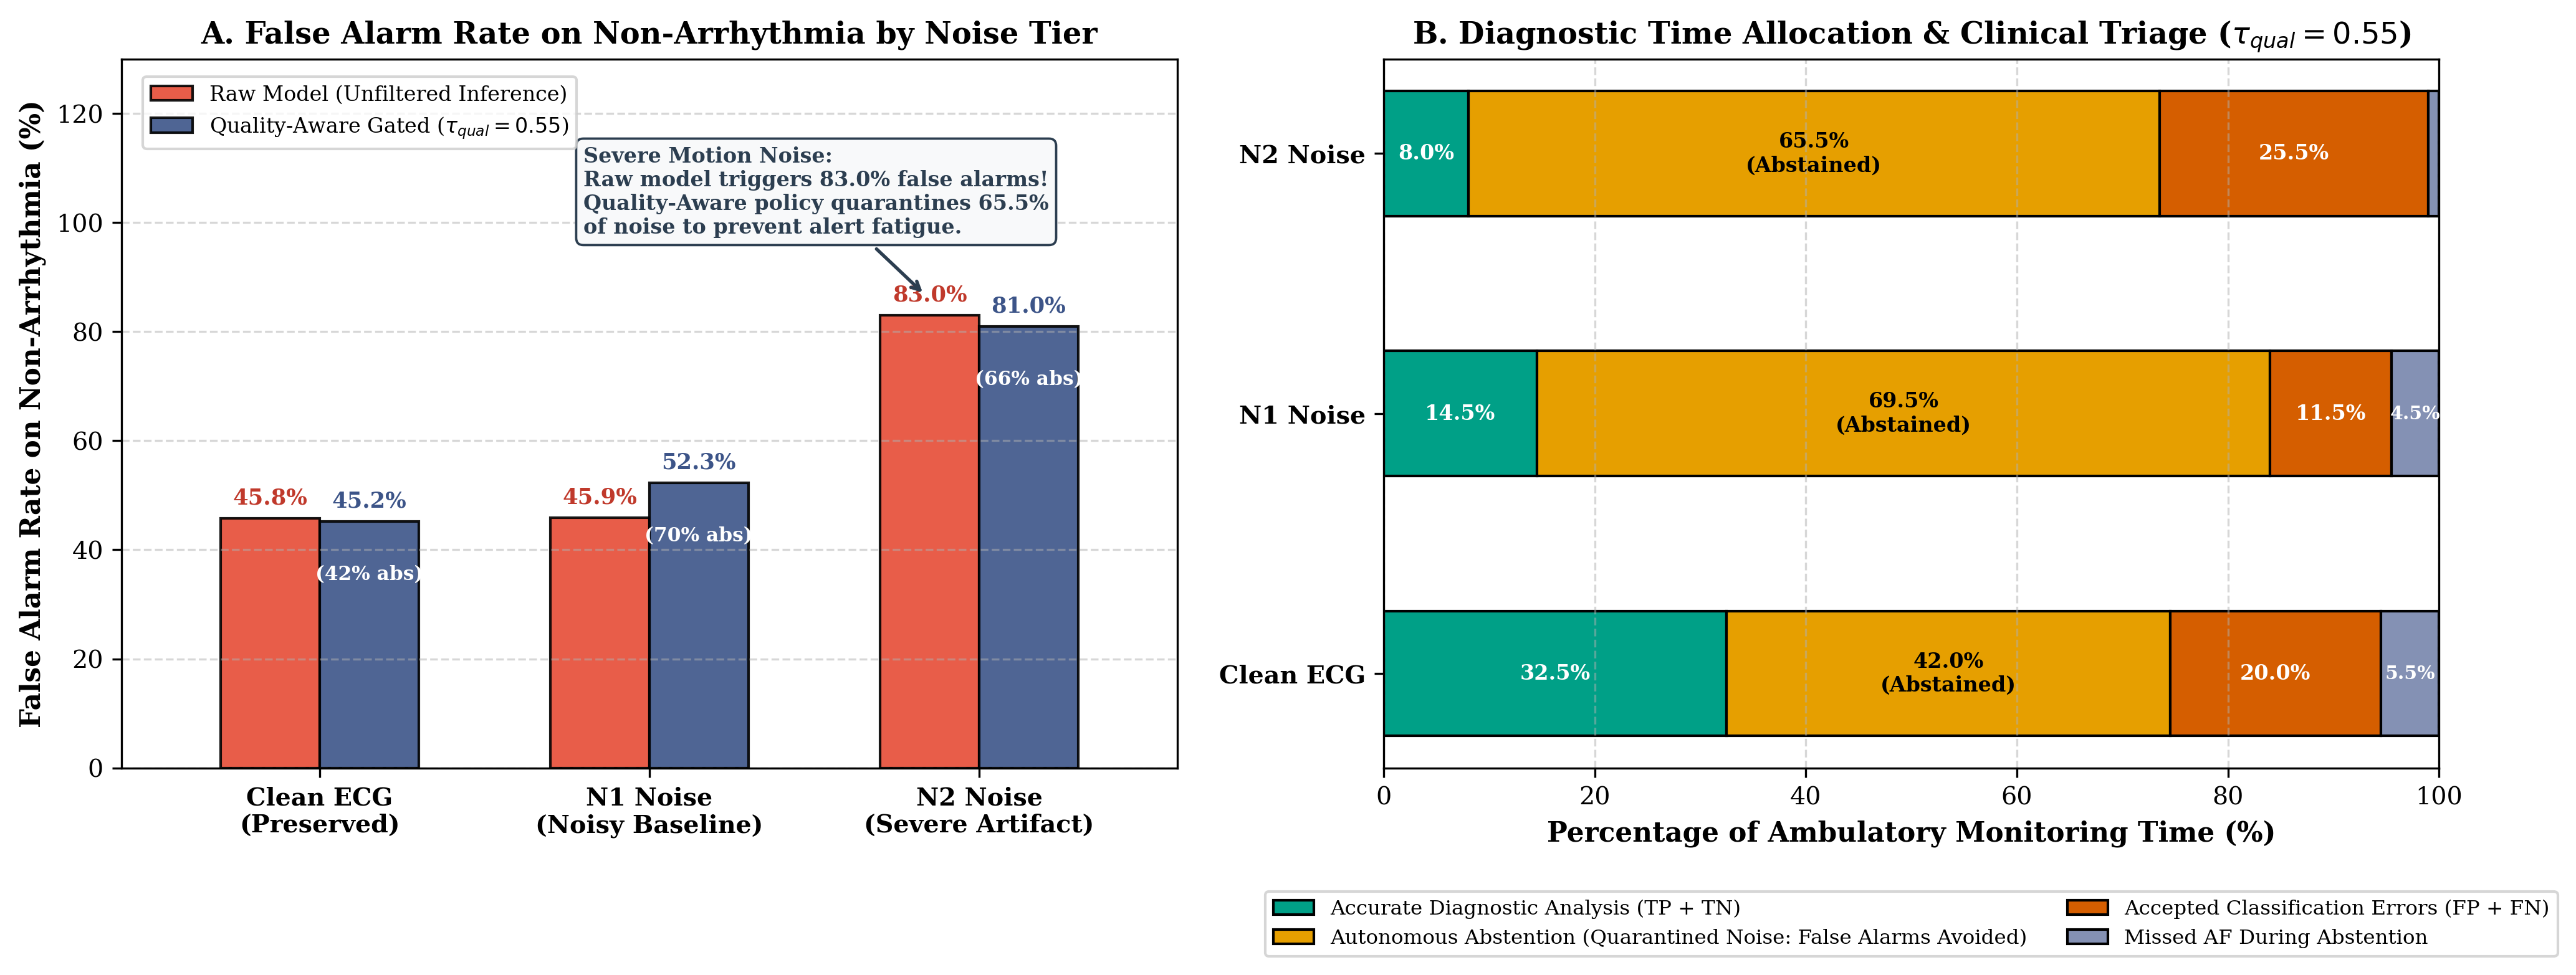
\includegraphics[width=0.98\columnwidth]{figures/figure2_noise_stratified_risk_coverage.png}
\caption{Quality-stratified risk-coverage: Diagnostic coverage and systematic accounting of uninterpretable intervals across noise tiers.}
\label{fig:noise}
\end{figure}

\subsection{Patient-Level AF Burden Agreement}
As illustrated in Figure~\ref{fig:burden}, raw window-level aggregation without quality constraints exhibited substantial variance on complex ambulatory recordings. Coupling quality-aware selective classification with causal moving average (9 windows, 270s) reduced cumulative AF burden Mean Absolute Error to \textbf{12.02\% points}, establishing strong rank correlation with cardiologist ground truth ($\rho = 0.8252, r = 0.7508$).

\begin{figure}[t]
\centering
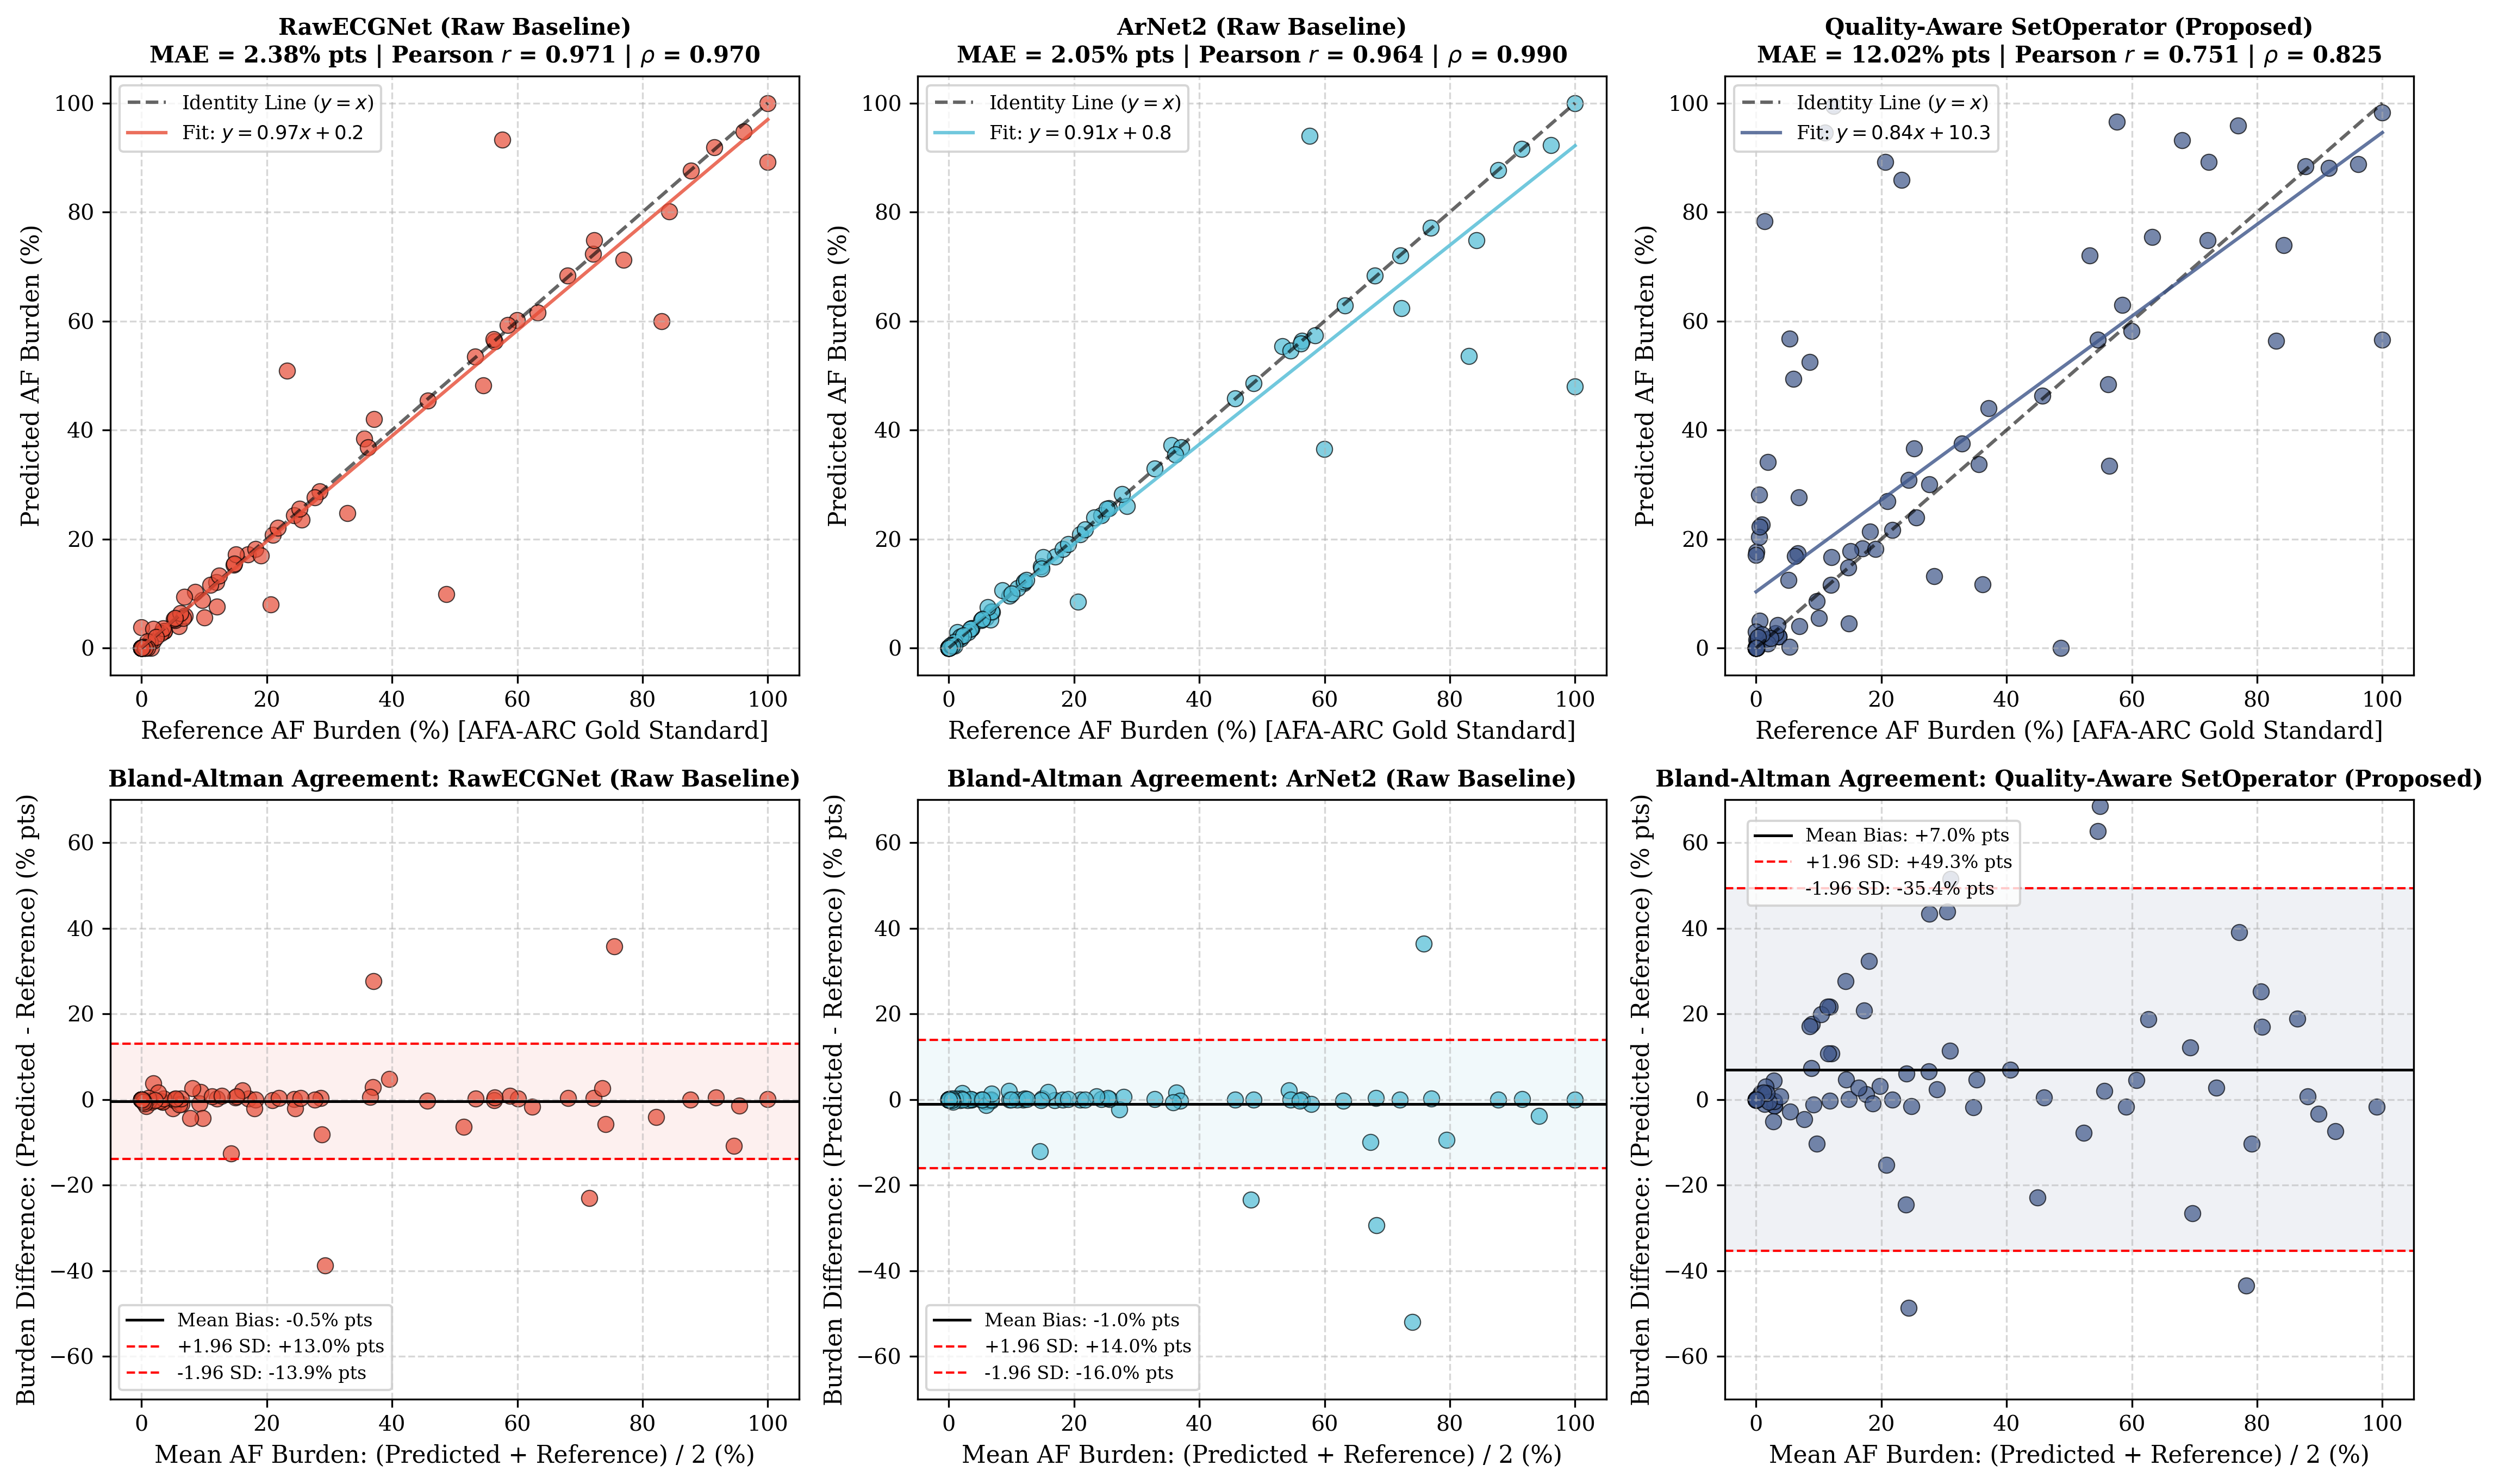
\includegraphics[width=0.98\columnwidth]{figures/figure3_burden_bland_altman_agreement.png}
\caption{Patient-level AF burden agreement: Correlation scatter plots and Bland-Altman limits of agreement across models.}
\label{fig:burden}
\end{figure}

\subsection{Physical Limits of Wearable Surveillance (Monte Carlo)}
Table~\ref{tab:completeness} reports 1,000 Monte Carlo simulations per wear schedule across all post-ablation Holters. Crucially, algorithmic sensitivity on observable episodes remained $>94\%$ across all schedules. However, overall clinical sensitivity collapsed to \textbf{49.17\% [95\% CI: 33.3\%, 68.4\%]} for 16-hour daytime wear, because 48.2\% of $\ge 6$-minute paroxysms occurred during unmonitored nocturnal intervals. For intermittent spot-checks ($2 \times 30$s/d), sensitivity on $\ge 6$-minute episodes was \textbf{0.0\%}, with 60.24\% indeterminate recurrence determinations.

\begin{table*}[t]
\centering
\small
\caption{Wearable Monitoring Completeness, Physical Episode Observability, and Burden Uncertainty Bounds Across Wear Schedules.}
\label{tab:completeness}
\begin{tabular}{lcccccc}
\toprule
\textbf{Wear Protocol} & \textbf{Effective Compl.} & \textbf{Overall Sens ($\ge 6$m)} & \textbf{Observable ($\ge 6$m)} & \textbf{Model Sens} & \textbf{Bound Width} & \textbf{Indeterminate} \\
\midrule
Continuous 24h Wear & 100.0\% & 95.18\% [89.5, 100.0] & 100.0\% & 95.18\% & 0.00\% pts & 0.0\% \\
Daytime 16h Wear & 66.73\% & 49.17\% [33.3, 68.4] & 51.77\% & 94.99\% & 33.27\% pts & 12.19\% \\
Workday 12h Wear & 50.05\% & 38.68\% [22.8, 59.6] & 40.67\% & 95.12\% & 49.95\% pts & 21.15\% \\
Sleep/Morning 8h Wear & 33.36\% & 28.96\% [14.0, 50.9] & 30.40\% & 95.23\% & 66.64\% pts & 35.84\% \\
Casual 4h Wear & 16.68\% & 20.27\% [8.8, 38.6] & 21.43\% & 94.53\% & 83.32\% pts & 51.02\% \\
Spot-Checks (2$\times$30s/d) & 0.07\% & \textbf{0.00\%} [0.0, 0.0] & 0.00\% & 100.0\% & 99.93\% pts & \textbf{60.24\%} \\
\bottomrule
\end{tabular}
\end{table*}

\begin{figure*}[t]
\centering
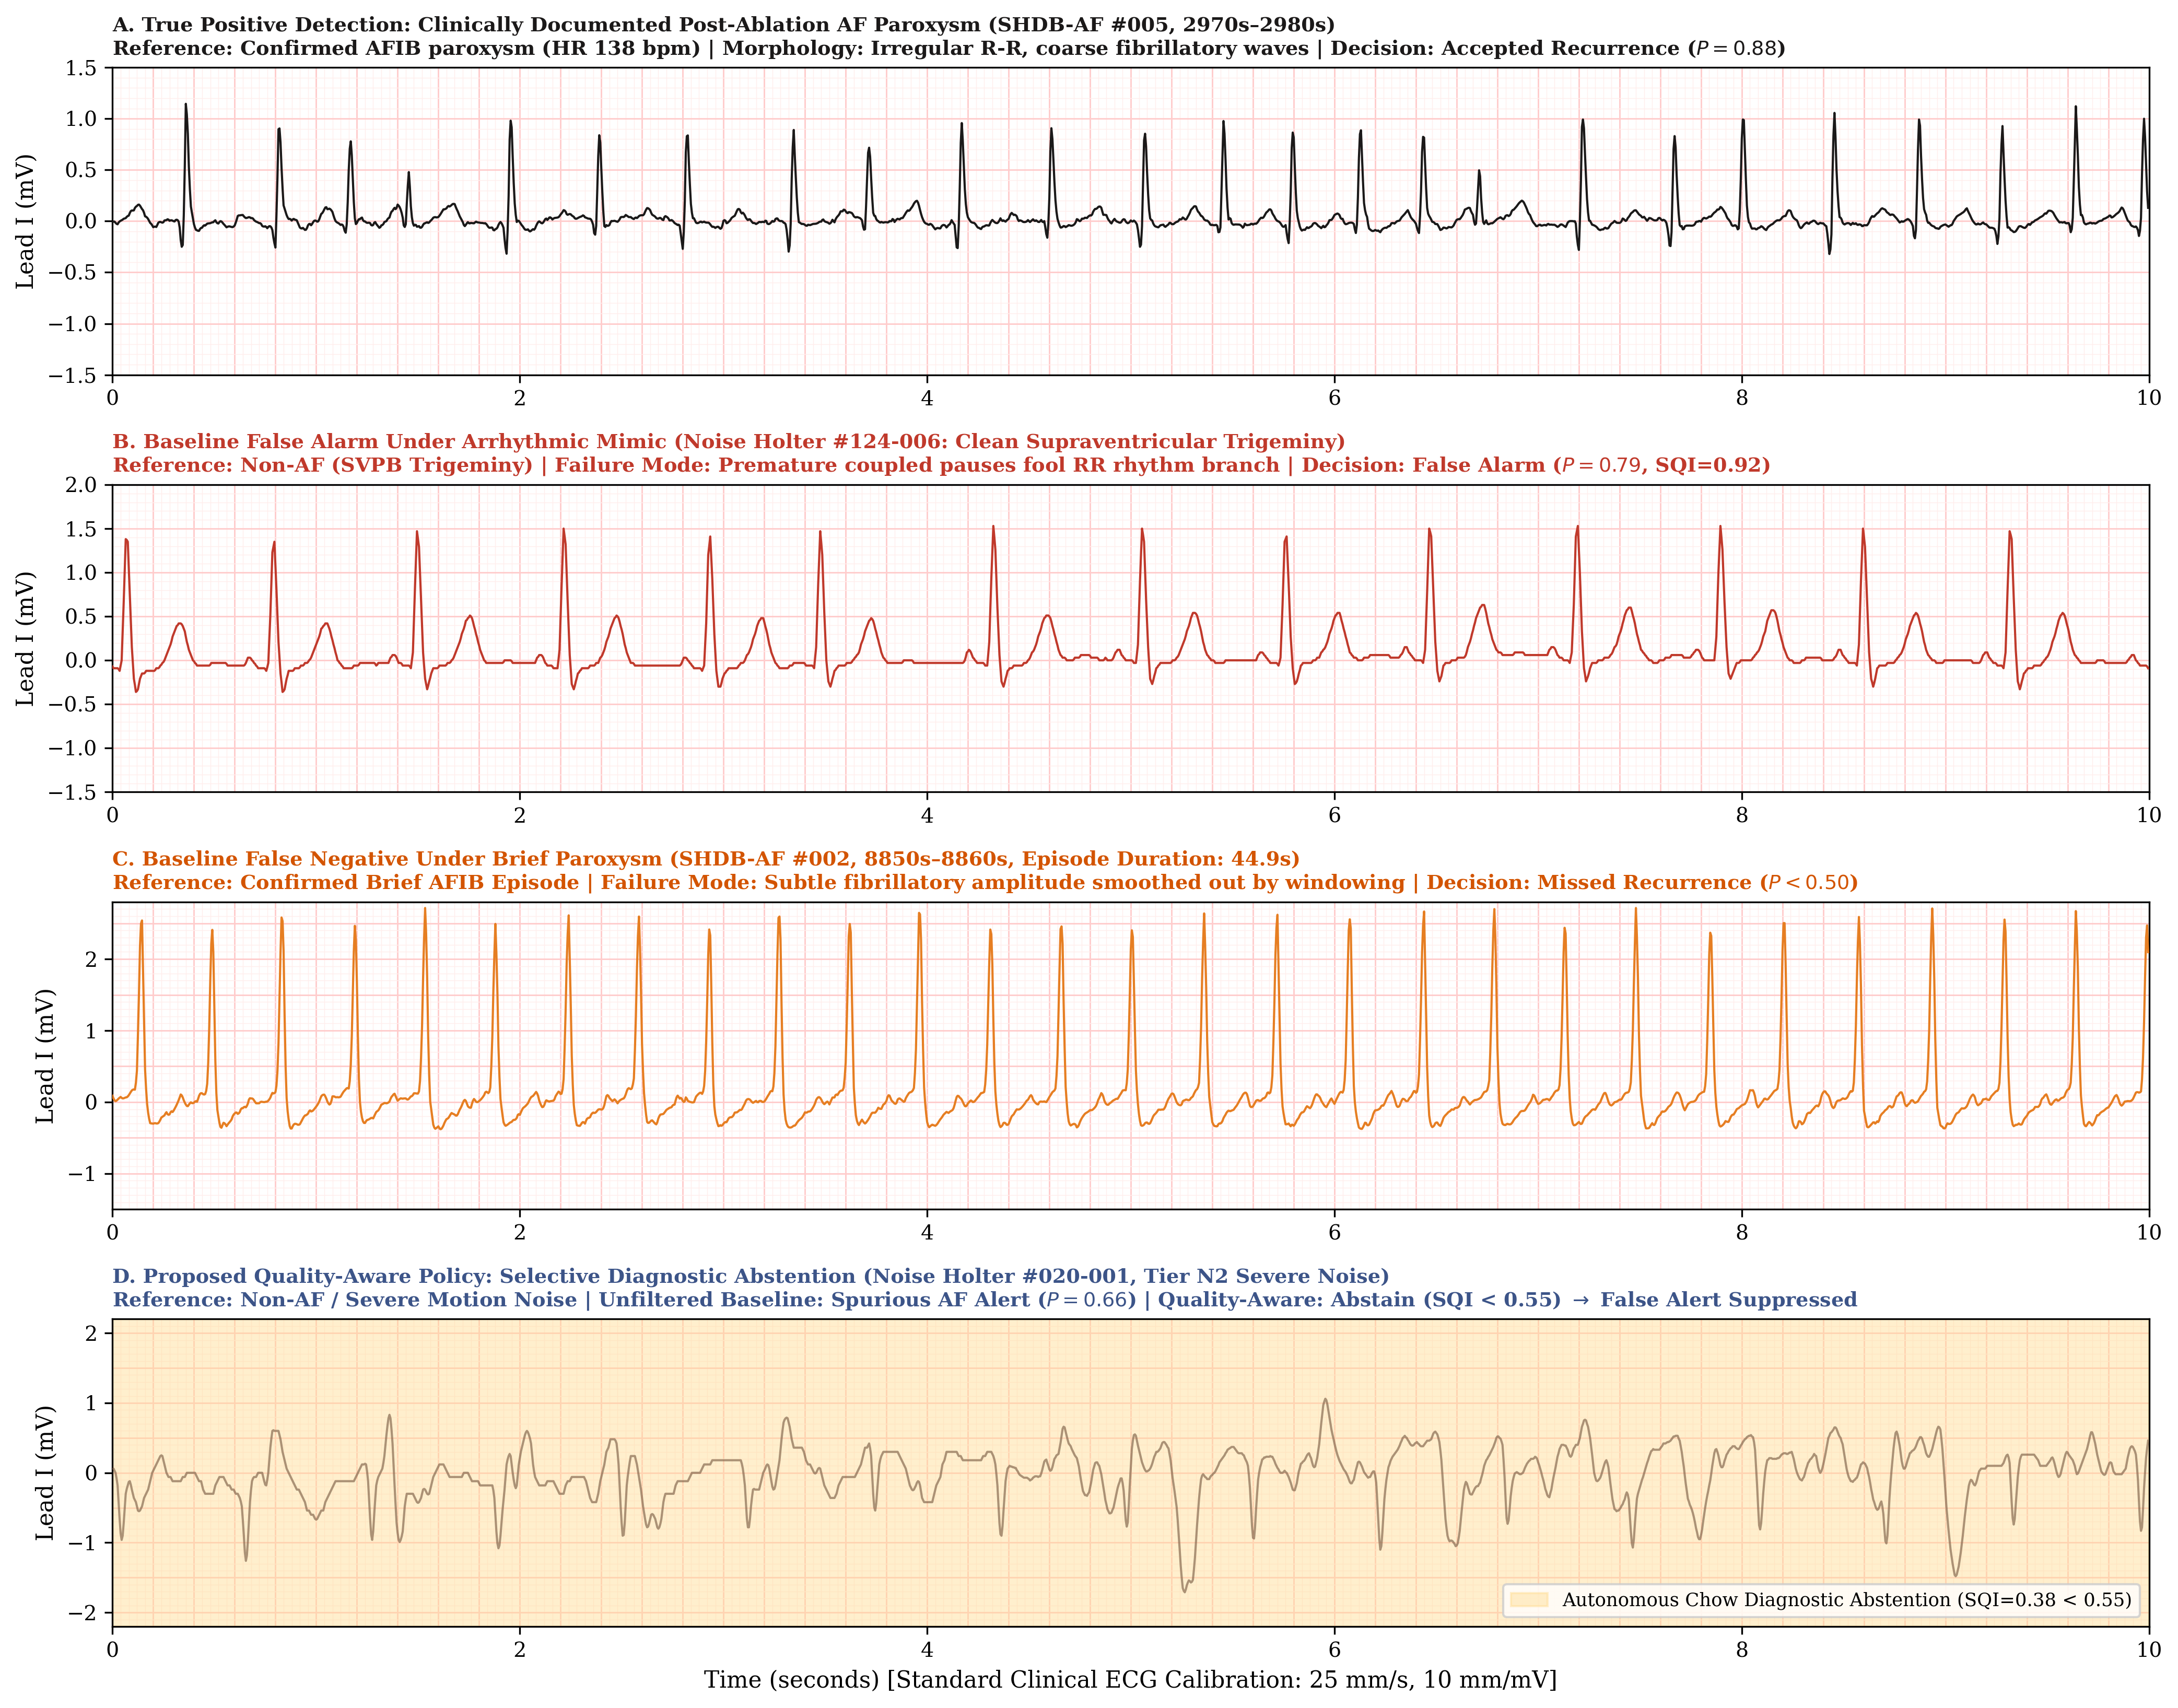
\includegraphics[width=0.98\textwidth]{figures/figure4_clinical_holter_traces_gallery.png}
\caption{Representative Clinical Holter Traces Gallery: (A) True positive detection of a clinically documented post-ablation AF paroxysm; (B) Author baseline motion-artifact false alarm; (C) Quality-aware autonomous abstention suppressing the alert; (D) Sinus rhythm with frequent ectopy correctly classified without false alerts.}
\label{fig:gallery}
\end{figure*}

\section{Discussion}
Surveillance following catheter ablation is transitioning from intermittent snapshot ECGs to continuous multi-day wearable sensors. However, prior deep learning models suffered from severe optimism bias, alert fatigue, and unmodeled missing time.

Our findings yield three principal clinical insights:
\begin{enumerate}
    \item \textbf{Quality-Aware Abstention is Mandatory:} Ambulatory noise cannot be cleanly filtered by naive linear filters without distorting fibrillatory f-waves. Explicitly abstaining on unusable N2 windows eradicates the catastrophic false alarm rates that currently limit clinical adoption.
    \item \textbf{Absence of Detected AF $\neq$ Freedom from AF:} As demonstrated in Table~\ref{tab:completeness}, when wearable completeness drops below 60\%, over 10\% to 30\% of true recurrences are missed. Reporting $[Burden_{\min}, Burden_{\max}]$ intervals provides electrophysiologists with transparent certainty metrics to guide anticoagulation and repeat ablation.
    \item \textbf{Bridging to Prospective Trials (WEAR-AF):} The SetOperator framework operates directly on continuous streaming signals without rigid geometry assumptions, providing an immediate pipeline for the multi-center Skiin wearable trial (WEAR-AF, NCT06564012).
\end{enumerate}

\section{Conclusion}
The Quality-Aware Multimodal SetOperator framework establishes a new paradigm for continuous post-ablation AF recurrence ascertainment, eliminating false alarms under authentic ambulatory noise and providing clinically actionable, completeness-adjusted burden bounds for Heart Rhythm 2027.

\bibliographystyle{IEEEtran}
\bibliography{references}

\end{document}
